%!TEX root = main.tex
%%%%%%%%%%%%%%%%%%%%%%%%%%%%%%%%%%%%%%%%%%%%%%%%%%%%%%%%%%%%%%%%%%%%%%%%%%%%%%%%

\section{Introduction}
\label{sec:introduction}

Today, HTTP Adaptive Streaming (HAS) is the dominant way of video delivery in the Internet. 
HAS is based on the wide-spread HTTP protocol and takes over its properties such as easy traversal of NAT-devices, firewall-friendliness, encryption in the shape of HTTPS and close-to-customer caching through content-delivery networks (CDNs).
In HAS, the video content is split into short chunks, e.g. 2 seconds, and each chunk is encoded into different quality levels.
The individual chunks are then made available on standard HTTP servers.
The location of the chunks and their encoding are given to the client through a manifest file.
At beginning of the playback, the streaming client first requests the manifest file. 
Afterward, it chooses the chunks according to its internal adaptation logic, for example based on current throughput or buffer level.
Dynamic Adaptive Streaming of HTTP (DASH) is an ISO standard which defines the structure and content of such a manifest file and is deployed by major content providers such as YouTube or Netflix.

As users are shifting away from traditional video broadcast consumption to individual content selection through streaming services, user expectations are also growing. 
The user expects the content to be available on all his devices and everywhere he goes. 
It is well known that stalling events and the video encoding bit-rate (i.e. the video resolution) have a significant impact on the acceptance rate and the Quality of Experience (QoE) \cite{casas2012youtube}.
Therefor, it is important for the service provider to develop a sophisticated adaptation logic which can prevent stalling events even when faced with bottle-necked or unstable Internet connections, such as cellular access or congested links in after-work hours.

In this paper we take a closer look at the behavior of the adaptation logic of YouTube.
In previous work we showed that YouTube's adaptation logic focuses strictly on the user, to the account of network efficiency.
In particular, we observed the behavior that in some situations the YouTube player discards its currently buffered content to re-download it in a higher quality level.
That way, the player can increase the average quality level shown to the user.
However, the overall efficiency decreases as the previously downloaded segments are lost.
Figure \ref{fig:request_schedule} shows a request schedule for one of the experiment runs.
The axis to the right shows the request video interval in playback time, e.g. the first 16s of the video.
The axis to the left shows when the time of request based on the experiment time, with 0 being the time the HTTP GET request was send to the server.
At first, the play requests one minute of the lowest quality level.
20 seconds into the experiment, the player revises its previously made decision, discards two of the low quality segments (i.e. 30 seconds of playback time) and starts to download a higher quality level instead.
The shaded areas in the figure illustrate where lower quality segments were discarded.

Based on a large experimental dataset with over 10.000 video views under congested conditions and a optimization problem formulation, we quantify the optimality gap of the deployed adaptation logic in terms of user experience.






what:

how

main contribution: we show there there is a lot of room for optimization for the used adaptation algorithms. Even if we completely avoid stalling events, a higher mean video quality is achievable in most cases. The number of resolution switches can be reduced.

structure


\begin{figure}[t]
\centering
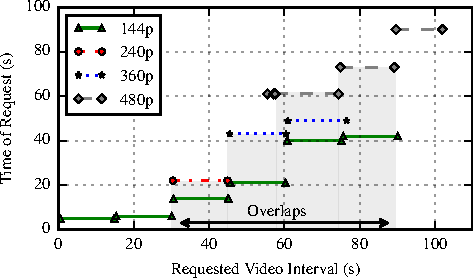
\includegraphics[width=0.9\linewidth]{figs/eg_request_schedule}%
\caption{Request schedule TODO: remake figure}
\label{fig:request_schedule}%
\end{figure}

\cite{sieber16sacrificing,sieber15costaggressive}